
\documentclass{standalone}
\usepackage[T1]{fontenc}
\usepackage[utf8]{inputenc}          % needed for French accents
\usepackage{pgfplotstable}
\usepackage{pgfplots}
\pgfplotsset{compat=1.18}
\usepackage{siunitx}                 % optional, nicer y‑axis numbers
\usepackage{booktabs}                % pretty tables for the optional preview

% -------------------------------------------------
% Helper that removes the internal \pgfpl@@ wrapper
% -------------------------------------------------

\begin{document}
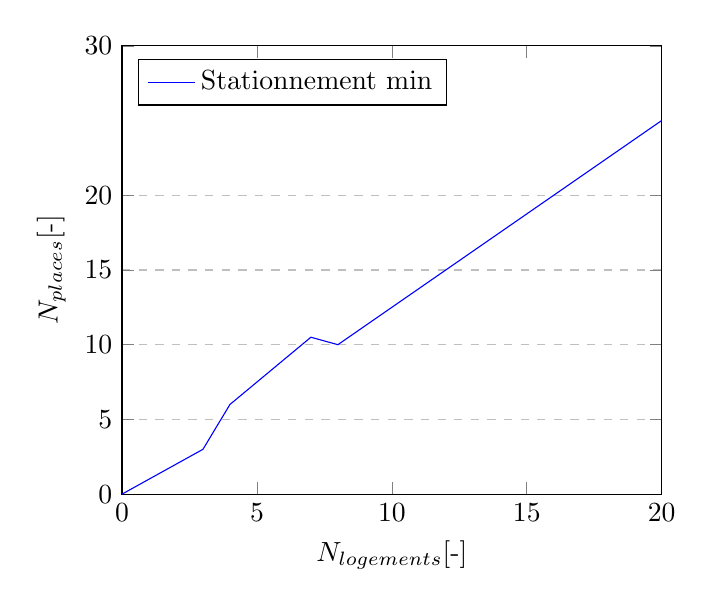
\begin{tikzpicture}[scale=1.0]
                \begin{axis}[
                    xlabel={$N_{logements}$[-]},
                    ylabel={$N_{places}$[-]},
                    xmin=0, xmax=20,
                    ymin=0, ymax=30,
                    xtick={0,5,10,15,20},
                    ytick={0,5,10,15,20,30},
                    legend pos=north west,
                    ymajorgrids=true,
                    grid style=dashed,
                ]
                \addplot[
                        color=blue
                        ]
                     coordinates {
                        (0,0)(3,3)(4,6)(5,7.5)(6,9)(7,10.5)(8,10)(10,12.5)(15,18.75)(20,25)
                    };
        
                \legend{Stationnement min}
                \end{axis}
            \end{tikzpicture}
        \end{document}